\chapauthor{Шункевич Д.В.\\Василевская А.П.\\Орлов М.К.\\Ивашенко В.П.}
\chapter{Смысловое представление логических формул и высказываний в различного вида логиках}
\chapauthortoc{Шункевич Д.В.\\Василевская А.П.\\Орлов М.К.\\Ивашенко В.П.}
\label{chapter_logic}

\begin{SCn}
	\begin{scnrelfromlist}{автор}
		\scnitem{Шункевич Д.~В.}
		\scnitem{Василевская А.~П.}
		\scnitem{Орлов М.~К.}
		\scnitem{Ивашенко В.~П.}
	\end{scnrelfromlist}
	
	\bigskip
	
	\scntext{аннотация}{В главе рассмотрено представление логических формул и высказываний как для классических логик и их приложений (прикладных логик), так и представление некоторых понятий неклассических логик.}
	
	\bigskip
	
	\begin{scnrelfromlist}{подраздел}
		\scnitem{\ref{sec_class_logic}~\nameref{sec_class_logic}}
		\scnitem{\ref{sec_applied_logic}~\nameref{sec_applied_logic}}
		\scnitem{\ref{sec_nonclass_logic}~\nameref{sec_nonclass_logic}}
	\end{scnrelfromlist}
	
	\bigskip
	
	\begin{scnrelfromlist}{ключевое понятие}
		\scnitem{логическая формула}
		\scnitem{атомарная логическая формула}
		\scnitem{неатомарная логическая формула}
		\scnitem{замкнутая логическая формула}
		\scnitem{открытая логическая формула}
		\scnitem{высказывание}
		\scnitem{атомарное высказывание}
		\scnitem{неатомарное высказывание}
		\scnitem{фактографическое высказывание}
		\scnitem{нефактографическое высказывание}
		\scnitem{атомарное фактографическое высказывание}
		\scnitem{атомарное нефактографическое высказывание}
		\scnitem{неатомарное нефактографическое высказывание}
		\scnitem{выполнимая логическая формула}
		\scnitem{невыполнимая логическая формула}
		\scnitem{общезначимая логическая формула}
		\scnitem{нейтральная логическая формула}				
		\scnitem{необщезначимая логическая формула}
		\scnitem{логическая формула, равнозначная логической константе}				
		\scnitem{атомарное существование}			
		\scnitem{кратность существования}			
		\scnitem{единственность существования}			
		\scnitem{иррефлексивное слотовое бинарное отношение}
		\scnitem{иррефлексивное неслотовое бинарное отношение}
		\scnitem{рефлексивное слотовое бинарное отношение}
		\scnitem{рефлексивное неслотовое бинарное отношение}
		\scnitem{транзитивное слотовое бинарное отношение}
		\scnitem{транзитивное неслотовое бинарное отношение}
		\scnitem{симметричное слотовое бинарное отношение}
		\scnitem{симметричное неслотовое бинарное отношение}
		\scnitem{антисимметричное слотовое бинарное отношение}
		\scnitem{антисимметричное неслотовое бинарное отношение}
		\scnitem{слотовое бинарное отношение}
		\scnitem{неслотовое бинарное отношение}
		\scnitem{слотовое отношение эквивалентности}
		\scnitem{неслотовое отношение эквивалентности}
		\scnitem{слотовое отношение нестрогого порядка}
		\scnitem{неслотовое отношение нестрогого порядка}
		\scnitem{секвенция}
		\scnitem{метаструктура}
		\scnitem{модальный оператор}
		\scnitem{модальное правило вывода}
		\scnitem{отношение становления структур}
		\scnitem{последовательность мышления}
		\scnitem{немонотонный вывод на конечном sc-множестве посылок}
		\scnitem{выводимое множество}
	\end{scnrelfromlist}
	
	\bigskip
	
	\begin{scnrelfromlist}{ключевое отношение}
		\scnitem{высказывание*}
		\scnitem{неразрешимое высказывание*}
		\scnitem{истинное высказывание*}
		\scnitem{ложное высказывание*}
		\scnitem{подформула*}				
		\scnitem{логическая связка*}				
		\scnitem{конъюнкция*}						
		\scnitem{дизъюнкция*}								
		\scnitem{отрицание*}
		\scnitem{строгая дизъюнкция*}	
		\scnitem{эквиваленция*}
		\scnitem{импликация*}
		\scnitem{если\scnrolesign}										
		\scnitem{то\scnrolesign}												
		\scnitem{квантор*}	
		\scnitem{всеобшность*}	
		\scnitem{существование*}	
		\scnitem{неатомарное существование*}
		\scnitem{нечёткая истинность*}
		\scnitem{конструктивно истинное высказывание*}
		\scnitem{верное высказывание*}
		\scnitem{монотонное бинарное отношение*}
		\scnitem{неискажённое высказывание*}
	\end{scnrelfromlist}

	\begin{scnrelfromlist}{ключевое знание}
		\scnitem{Описание понятия формальной теории}
		\scnitem{Описание понятия утверждения}				
		\scnitem{Описание понятия определение}
	\end{scnrelfromlist}
	
	\bigskip
	
	\begin{scnrelfromlist}{ключевой знак}
		\scnitem{Отношение выводимости}
		\scnitem{Отношение выводимости на конечных множествах}
		\scnitem{Отношение выводимости на конечных множествах полносвязно представленных множеств}
		\scnitem{Отношение выводимости на секвенциях}
	\end{scnrelfromlist}
	
	\bigskip
	
	\begin{scnrelfromlist}{библиографическая ссылка}
		\scnitem{\scncite{Letichevskij2003}}
		\scnitem{\scncite{Klini1973}}
		\scnitem{\scncite{Gribomon1990}}
		\scnitem{\scncite{Gribomon1998}}
		\scnitem{\scncite{Dragalin}}
		\scnitem{\scncite{Vagin2008}}
		\scnitem{\scncite{Golenkov2001b}}
		\scnitem{\scncite{Tarasov2007}}
		\scnitem{\scncite{Cintula2011}}		
		\scnitem{\scncite{Ivashenko2014diss}}
		\scnitem{\scncite{Ivashenko2017}}
	\end{scnrelfromlist}
	
\end{SCn}

%Перенесено из chapter_logic_productions
%Язык SCL является логическим языком графового типа, используемым ostis-системами. Тексты языка SCL представляют собой однородные семантические сети, являющиеся текстами языка SC. Алфавит языка SCL отдельно не выделяется, так как используется алфавит SC-кода, на котором можно описать любые утверждения, явления, закономерности, программы и любые другие знания. Язык SCL позволяет записывать тексты языка логики высказываний, языка логики предикатов и любых других логических языков. SC-код является метаязыком как для языка SCL, так и для самого себя, то есть он позволяет описывать смысл формул, записанных на SCL. Многие формальные языки, в отличие от SC, недостаточно богаты, чтобы быть метаязыком для самих себя. 

%Одной из важных особенностей SCL является его способность представления текстов языка логики предикатов с учётом семантики этих текстов (высказываний). Язык SCL естественным образом ориентирован на работу в формальной системе языка логики предикатов. Язык SC позволяет записать любые отношения и соответствия в графовом представлении. Значению предиката от некоторого набора sc-переменных соответствует результат операции поиска по шаблону некоторой sc-конструкции (найдена или не найдена), в которую входят sc-константы и/или sc-переменные с соответствующей конфигурацией связей между ними. Подход, основанный на языке SCL для представления формул предоставляет возможность явно не записывать кванторы общности и существования (это не запрещается, однако является излишним). Квантор существования является "встроенным"{} понятием в том смысле, что если некоторый sc-элемент входит в некоторую sc-структуру, то соответствующее понятие существует в этой sc-структуре. Таким образом, квантор существования накладывается автоматически (если иной квантор не наложен явно) на те sc-переменные, которые входят в атомарные логические формулы. Квантор всеобщности накладывается по умолчанию (если иной квантор не наложен явно) на переменные, входящие в связки эквиваленции и импликации в соответствии с денотационной семантикой логических языков.

% Вагин дедукция и обобщения в системах принятия решений
\section{Смысловое представление логических формул и формальных теорий классической логики}
\label{sec_class_logic}
Появление \textit{формальных систем} было обусловлено осознанием того факта, что совершенно различные системы, будь то технические, социальные, экономические или биологические, обладают глубоким сходством. Действительно, каждая конкретная система состоит из каких-то первичных (базовых) элементов, обладающих какими-то свойствами. Затем, исходя из наличия исходных описаний, можно логическим путём вывести описание новых свойств, причём утверждения о наличии исходных или выведенных свойств воспринимаются как истинные на основании смысла определений данных элементов.

\scnkeyword{формальная теория} --- это \textit{множество} \textit{высказываний}, которые считаются истинными в рамках данной \scnkeyword{формальной теории}.

Аксиоматические системы --- это системы с наличием определённого числа исходных заранее выбранных и фиксированных высказываний, называемых аксиомами.

\textit{высказывания} могут быть как фактографическими, так и нефактографическими. Некоторые \textit{высказывания} считаются аксиомами, а другие доказываются на основе других высказываний в рамках этой же \scnkeyword{формальной теории}.

Каждая формальная теория интерпретируется (то есть ее \textit{высказывания} являются истинными) на какой-либо \textit{предметной области}, которая является максимальным из \textit{фактографических высказываний} (их \textit{объединением*}),  входящих в состав этой \scnkeyword{формальной теории}.

Каждой \scnkeyword{формальной теории} соответствует одна \textit{предметная область}, которая входит в нее под атрибутом \textit{предметная область\scnrolesign}.

Каждая \textit{формальная теория} может рассматриваться как \textit{конъюнктивное высказывание}, априори истинное (с чьей-то точки зрения) при интерпретации на соответствующей предметной области.

Каждая \textit{формальная теория} задаётся \textit{алфавитом}, \textit{формулами}, \textit{аксиомами}, \textit{правилами вывода}.

%\scnrelfrom{источник}{\scncite{Serhievskaya2004}}

\textit{предметная область} является \textit{максимальным фактографическим высказыванием} \textit{формальной теории}, которая интерпретируется на данной \textit{предметной области}.

\textbf{\textit{аксиома}} --- это \textit{высказывание}, истинность которого не требует доказательства в рамках рассматриваемой \textit{формальной теории}.

\textbf{\textit{теорема}} --- это \textit{высказывание}, истинность которого доказывается в рамках рассматриваемой \textit{формальной теории}.

\begin{SCn}
\scnheader{логическая формула}
\begin{scnrelfromset}{разбиение}
	\scnitem{атомарная логическая формула}
	\scnitem{неатомарная логическая формула}
\end{scnrelfromset}
\begin{scnrelfromset}{разбиение}
	\scnitem{замкнутая логическая формула}
	\scnitem{открытая логическая формула}
\end{scnrelfromset}
\end{SCn}
\begin{SCn}
\scnheader{высказывание}
\scnsubset{логическая формула}
\begin{scnrelfromset}{разбиение}
	\scnitem{атомарное высказывание}
	\scnitem{неатомарное высказывание}
\end{scnrelfromset}
\begin{scnrelfromset}{разбиение}
	\scnitem{фактографическое высказывание}
	\begin{scnindent}
		\scnsubset{замкнутая логическая формула}
	\end{scnindent}
	\scnitem{нефактографическое высказывание}
\end{scnrelfromset}
\end{SCn}

Под \textbf{\textit{высказыванием}} понимается некоторая \textit{структура} (в которую входят \textit{sc-константы} из некоторой предметной области и/или \textit{sc-переменные}) или \textit{логическая связка}, которая может трактоваться как истинная или ложная в рамках какой-либо \textit{предметной области}.

Истинность \textbf{\textit{высказывания}} задаётся путем указания принадлежности знака этого высказывания \textit{формальной теории}, соответствующей данной \textit{предметной области}. Ложность высказывания задается путем указания принадлежности знака \textit{отрицания*} этого высказывания данной \textit{формальной теории}.

Явно указанная непринадлежность \textbf{\textit{высказывания}} \textit{формальной теории} может говорить как о его ложности в рамках данной теории (если это указано рассмотренным выше образом), так и о том, что данное  \textbf{\textit{высказывание}} вообще не рассматривается в данной \textit{формальной теории} (например, использует понятия, не принадлежащие данной \textit{предметной области}).

Одно и то же \textbf{\textit{высказывание}} может быть истинно в рамках одной \textit{формальной теории} и ложно в рамках другой.

%\begin{SCn}
%% Добавить темпоральное высказывание
%\scnheader{высказывание формальной теории\scnrolesign}
%\begin{scnrelfromset}{разбиение}
%	\scnitem{истинное высказывание\scnrolesign}
%	\scnitem{ложное высказывание\scnrolesign}
%%	\scnitem{нечеткое высказывание\scnrolesign}
%	\scnitem{бессмысленное высказывание\scnrolesign}
%\end{scnrelfromset}
%\end{SCn}

%\textbf{\textit{истинное высказывание}} --- высказывание, знак которого принадлежит изучаемой формальной теории.
%Нечеткое высказывание --- высказывание, возможно истинное или ложное в рамках изучаемой формальной теории (высказывание, возможно истинное или ложное в рамках данной формальной теории).
%\textbf{\textit{бессмысленное высказывание}} --- высказывание, не рассматриваемое в рамках данной формальной теории. Высказывание является бессмысленным в рамках заданной формальной теории, если в какое-либо \textit{атомарное высказывание} в его составе (или в само это высказывание, если оно является атомарным) входит какая-либо \textit{sc-константа}, не являющаяся элементом предметной области, описываемой указанной \textit{формальной теорией}.

\begin{SCn}
\scnheader{атомарное высказывание}
\scnsubset{структура}
\begin{scnrelfromset}{разбиение}
	\scnitem{атомарное фактографическое высказывание}
	\scnitem{атомарное нефактографическое высказывание}
\end{scnrelfromset}
\end{SCn}

\textbf{\textit{атомарное высказывание}} --- это \textit{высказывание}, которое не является \textit{неатомарным высказыванием}.

\textbf{\textit{неатомарное высказывание}} --- это \textit{высказывание}, в состав которого входят только знаки \textit{логических формул} или множества связываемых переменных. Следует отметить, что невозможно говорить об истинности либо ложности \textbf{\textit{неатомарного высказывания}} в рамках какой-либо \textit{формальной теории}, в случае, когда невозможно установить истинность либо ложность любого из его элементов в рамках этой же \textit{формальной теории} или интерпретации этих элементов.

Под \textit{фактографическим высказыванием} понимается:
\begin{textitemize}
	\item \textit{атомарное высказывание}, в состав которого не входит ни одна \textit{sc-переменная};
	\item \textit{неатомарное высказывание}, все элементы которого также являются \textbf{\textit{фактографическими высказываниями}}.
\end{textitemize}

\begin{SCn}
\scnheader{высказывание*}
\scnidtf{бинарное ориентированное отношение, каждая \textit{пара} которого связывает (1) знак некоторой \textit{предметной области} и (2) знак некоторого \textit{высказывания}.}
\begin{scnrelfromset}{разбиение}
	\scnitem{ложное высказывание*}
	\scnitem{неразрешимое высказывание*}
%	\begin{scnindent}
%			\scnsuperset{гипотеза}
%	\end{scnindent}}
	\scnitem{истинное высказывание*}	
\end{scnrelfromset}
\end{SCn}

%\scntext{предъявляемое требование}{Все \textit{sc-элементы}, входящие в состав \textit{предметной области}, описываемой высказыванием, (включая и \textit{sc-переменные}, которые, хоть и редко, но могут входить в состав некоторых \textit{предметных областей}) 
%\textit{sc-элементами} для всех высказываний, соответствующих этой \textit{предметной области}.}

\scntext{предъявляемое требование}{Все \textit{sc-константы}, входящие в состав всех \textit{атомарных логических формул}, входящих в состав всех \textit{высказываний}, описывающих некоторую \textit{предметную область} должны входить в состав описываемой \textit{предметной области}.}

\begin{SCn}
\scnheader{следует отличать*}
\begin{scnhaselementset}
	\scnitem{высказывание*}
	\begin{scnindent}
		\scniselement{бинарное ориентированное отношение}
		\scnidtf{быть высказыванием, описывающим заданную предметную область*}
		\begin{scnindent}
			\scntext{сокращение}{быть высказыванием*}
		\end{scnindent}
	\end{scnindent}
	\scnitem{высказывание}
	\begin{scnindent}
		\scnsubset{логическая формула}
		\scnidtf{Второй домен отношения ``быть высказыванием''}
	\end{scnindent}
\end{scnhaselementset}
\end{SCn}

\begin{SCn}
\scnheader{нефактографическое высказывание}
\begin{scnrelfromset}{разбиение}
	\scnitem{атомарное нефактографическое высказывание}
	\scnitem{неатомарное нефактографическое высказывание}
\end{scnrelfromset}
\end{SCn}

Под \textit{нефактографическим высказыванием} понимается:
\begin{textitemize}
	\item \textit{атомарное нефактографическое высказывание}, в состав которого входит хотя бы одна \textit{sc-переменная};
	\item \textit{неатомарное нефактографическое высказывание}, хотя бы один элемент которого является \textbf{\textit{нефактографическим высказыванием}}.
\end{textitemize}

Под \textbf{\textit{атомарным нефактографическим высказыванием}} понимается \textit{атомарное высказывание}, которое является \textit{нефактографическим высказыванием}.

\textbf{\textit{атомарное нефактографическое высказывание}} --- это \textit{нефактографическое высказывание}, которая не является \textit{неатомарным нефактографическим высказыванием}.

\textbf{\textit{атомарная логическая формула}} --- это \textit{логическая формула}, которая не является \textit{неатомарной логической формулой}.

По умолчанию \textbf{\textit{атомарное нефактографическое высказывание}} трактуется как \textit{высказывание} о существовании, то есть наличия в памяти значений, соответствующих всем \textit{sc-переменным}, входящим в состав данной формулы и не попадающих под действие какого-либо другого \textit{квантора} (указанного явно или по умолчанию). Таким образом, на все \textit{sc-переменные}, входящие в состав \textit{атомарного нефактографического высказывания} и не попадающие под действие какого-либо другого \textit{квантора}, неявно накладывается квантор \textit{существования*}.

\begin{SCn}
\scnheader{логическая формула}
\begin{scnrelfromset}{разбиение}
	\scnitem{выполнимая логическая формула}
	\begin{scnindent}
		\begin{scnrelfromset}{разбиение}
			\scnitem{общезначимая логическая формула}
			\scnitem{нейтральная логическая формула}
		\end{scnrelfromset}
	\end{scnindent}
	\scnitem{невыполнимая логическая формула}
\end{scnrelfromset}
\end{SCn}

Под \textbf{\textit{неатомарным нефактографическим высказыванием}} понимается \textit{неатомарное высказывание}, которое является \textit{нефактографическим высказыванием}.

Для того, чтобы рассмотреть типологию \textbf{\textit{неатомарных логических формул}}, будем говорить, что исследуется истинность самой \textbf{\textit{неатомарной логической формулы}} и всех ее \textit{подформул*} в рамках одной и той же \textit{формальной теории}, при этом не важно, какой именно. Также считается, что в рассматриваемой \textit{формальной теории} каждая \textit{подформула*} рассматриваемой \textbf{\textit{неатомарной логической формулы}} в рамках этой \textit{формальной теории} может однозначно трактоваться как либо истинная, либо ложная. В противном случае мы не можем говорить об истинности либо ложности исходной \textbf{\textit{неатомарной логической формулы}} в рамках этой \textit{формальной теории}.

Будем называть \textbf{\textit{подформулой*}} \textit{неатомарной логической формулы} \textbf{\textit{fi}} любую \textit{логическую формулу} \textbf{\textit{fj}}, являющуюся элементом исходной формулы \textbf{\textit{fi}}, а также любую \textbf{\textit{подформулу*}} формулы \textbf{\textit{fj}}.

\begin{SCn}
\scnheader{подформула*}
\scnidtf{частная формула*}
\scniselement{бинарное отношение}
\scniselement{ориентированное отношение}
\scniselement{транзитивное отношение}
%\scnrelfrom{описание примера}{\scnfileitem{figures/sd_logical_formulas/subformula.png}}
\end{SCn}

\begin{figure}[H]
	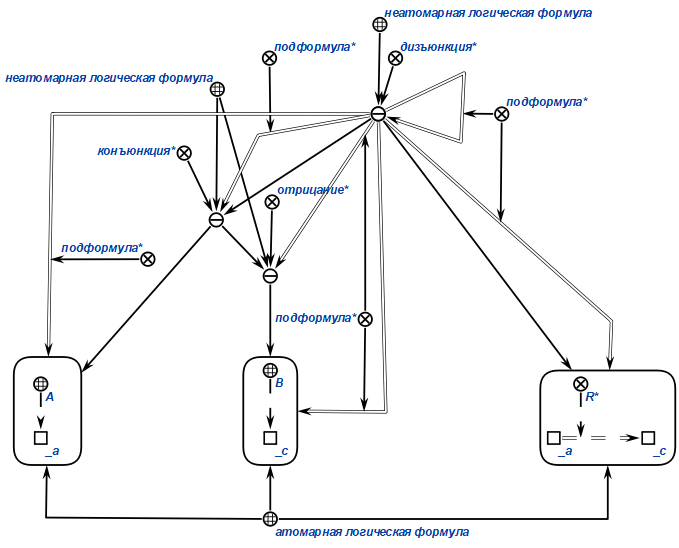
\includegraphics[scale=0.8]{author/part2/figures/logic/subformula.png}
	\caption{Формализация примера подформулы}
	\label{fig:modus_ponens}
\end{figure}

\textbf{\textit{утверждение}} --- это \textit{семантическая окрестность} некоторой \textit{логической формулы}, в которую входит полный текст этой \textit{логической формулы}, а также факт принадлежности этой \textit{логической формулы} некоторой \textit{формальной теории}.

Знак \textit{логической формулы}, семантическая окрестность которой представляет собой утверждение, является \textit{главным ключевым sc-элементом\scnrolesign} в рамках этого \textbf{\textit{утверждения}}. Знаки понятий соответствующей \textit{предметной области}, которые входят в состав какой-либо \textit{подформулы*} указанной \textit{логической формулы}, будут \textit{ключевыми sc-элементами\scnrolesign} в рамках этого \textbf{\textit{утверждения}}.
	
Полный текст некоторой \textit{логической формулы} включает в себя:
\begin{textitemize}
	\item{знак самой этой \textit{логической формулы}};
	\item{знаки всех ее \textit{подформул*}};
	\item{элементы всех \textit{логических формул}, знаки которых попали в данную структуру;}
	\item{все пары принадлежности, связывающие \textit{логические формулы}, знаки которых попали в данную структуру, с их компонентами.}
\end{textitemize}

Таким образом, факт принадлежности (истинности) логической формулы нескольким \textit{формальным теориям} будет порождать новое утверждение для каждой такой \textit{формальной теории}. Текст \textbf{\textit{утверждения}} входит в состав \textit{логической онтологии}, соответствующей \textit{предметной области}, на которой интерпретируется \textit{главный ключевой sc-элемент\scnrolesign} данного утверждения.

Правило идентификации экземпляров \textbf{\textit{утверждения}} в рамках \textit{Русского языка} именуются по следующим правилам:
\begin{textitemize}
	\item{в начале идентификатора пишется сокращение \textbf{Утв.};}
	\item{далее в круглых скобках через точку с запятой перечисляются основные идентификаторы \textit{ключевых \mbox{sc-элементов}\scnrolesign} данного \textbf{\textit{утверждения}}. Порядок определяется в каждом конкретном случае в зависимости от того, свойства каких из этих \textit{понятий} описывает данное \textbf{\textit{утверждение}} в большей или меньшей степени.}
\end{textitemize}

%\scntext{описание примера}{\textit{Утв. (параллельность*; секущая*)}}
Могут быть исключения для \textbf{\textit{утверждений}}, названия которых закрепились исторически, например, \textit{Теорема Пифагора}, \textit{Аксиома о прямой и точке}.


%\scnrelfrom{описание примера}{\scnfilescg{figures/sd_logical_formulas/statement.png}}
%Утверждение показывает, что соответствующие углы при пересечении параллельных прямых секущей равны.

\textbf{\textit{определение}} --- это \textit{утверждение}, \textit{главным ключевым sc-элементом\scnrolesign} которого является связка \textit{эквиваленции*}, однозначно определяющая некоторое понятие на основе других понятий.

Каждое определение имеет ровно один \textit{ключевой sc-элемент\scnrolesign} (не считая \textit{главного ключевого sc-элемента\scnrolesign}).

Для одного и того же понятия в рамках одной \textit{формальной теории} может существовать несколько \textit{утверждений об эквиваленции*}, однозначно задающих некоторое понятие на основе других, однако только одно такое \textit{утверждение} в рамках этой \textit{формальной теории} может быть отмечено как \textbf{\textit{определение}}. Остальные \textit{утверждения об эквиваленции*} могут трактоваться как \textit{пояснения} данного понятия.

Правило идентификации экземпляров \textbf{\textit{определения}} в рамках \textit{Русского языка} именуются по следующим правилам:
\begin{textitemize}
	\item{в начале идентификатора пишется сокращение \textbf{Опр.};}
	\item{далее в круглых скобках через точку с запятой записывается основной идентификатор  \textit{ключевого sc-элемента\scnrolesign} данного \textbf{\textit{определения}}.}
\end{textitemize}


%\scntext{описание примера}{\textit{Опр. (ромб)}}
%\scnrelfrom{описание примера}{\scnfilescg{figures/sd_logical_formulas/definition.png}}
%\scnnote{Определение показывает, что ромб — это четырёхугольник, у которого все стороны равны.}
\begin{SCn}
\scnheader{общезначимая логическая формула}
\scnidtf{тождественно истинная логическая формула}
\scnsubset{выполнимая логическая формула}
\scnsubset{логическая формула, равнозначная логической константе}
\end{SCn}
% Вагин, дедукция и обобщение в системах принятия решений
\textbf{\textit{общезначимая логическая формула}} --- это \textit{логическая формула}, для которой не существует \textit{формальной теории}, в рамках которой она была бы ложной (или имела бы ложную интерпретацию) с учетом истинности и ложности всех ее \textit{подформул*} (или их интерпретаций) в рамках этой же \textit{формальной теории}.

\begin{figure}[H]
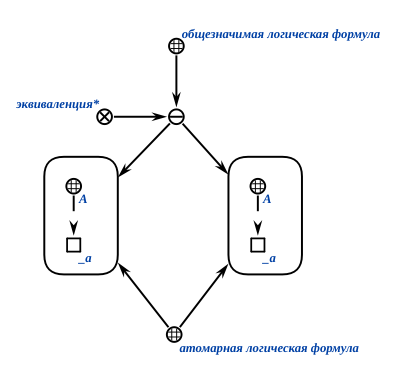
\includegraphics[scale=0.8]{author/part2/figures/logic/valid_formula.png}
\caption{Формализация закона тождества}
\label{fig:valid_formula}
\end{figure}

\begin{SCn}
\scnheader{противоречивая логическая формула}
\scnidtf{тождественно ложная логическая формула}
\scnsubset{невыполнимая логическая формула}
\scnsubset{логическая формула, равнозначная логической константе}
\end{SCn}
% Вагин, дедукция и обобщение в системах принятия решений
\textbf{\textit{противоречивая логическая формула}} --- это \textit{логическая формула}, для которой не существует \textit{формальной теории}, в рамках которой она была бы истинной (или имела бы истинную интерпретацию) с учетом истинности и ложности всех ее \textit{подформул*} (или их интерпретаций) в рамках этой же \textit{формальной теории}.

\begin{figure}[H]
	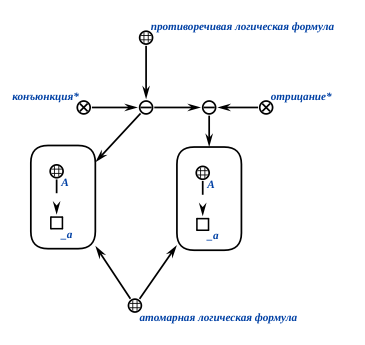
\includegraphics[scale=0.8]{author/part2/figures/logic/contradiction_formula.png}
	\caption{Формализация закона противоречия}
	\label{fig:contradiction_formula}
\end{figure}

\begin{SCn}
\scnheader{нейтральная логическая формула}
\scnsubset{выполнимая логическая формула}
\end{SCn}

\textbf{\textit{нейтральная логическая формула}} --- это \textit{логическая формула}, для которой существует хотя бы одна \textit{формальная теория}, в рамках которой эта формула ложна (или имеет ложную интерпретацию), и хотя бы одна \textit{формальная теория}, в рамках которой эта формула истинна (или имеет ложную интерпретацию).

\begin{figure}[H]
	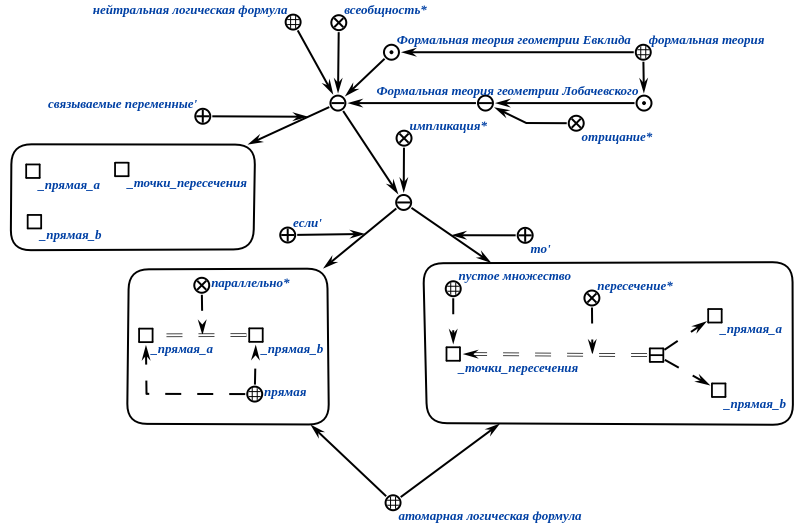
\includegraphics[scale=0.8]{author/part2/figures/logic/neutral_formula.png}
	\caption{Формализация нейтральной логической формулы}
	\label{fig:neutral_formula}
\end{figure}

В \textit{Геометрии Евклида} в плоскости через точку, не лежащую на данной прямой, можно провести одну и только одну прямую, параллельную данной. В \textit{Геометрии Лобачевского} данный постулат является ложным.
В \textit{Сферической геометрии} все прямые пересекаются.

\begin{SCn}
\scnheader{непротиворечивая логическая формула}
\scnidtf{выполнимая логическая формула}
\begin{scnreltoset}{объединение}
	\scnitem{нейтральная логическая формула}
	\scnitem{общезначимая логическая формула}
\end{scnreltoset}
\end{SCn}

\textbf{\textit{непротиворечивая логическая формула}} --- это \textit{логическая формула}, для которой существует хотя бы одна \textit{формальная теория}, в рамках которой эта формула истинна (или имеет истинную интерпретацию).

\begin{SCn}
\scnheader{необщезначимая логическая формула}
%\scnidtf{невыполнимая логическая формула}
\begin{scnreltoset}{объединение}
	\scnitem{нейтральная логическая формула}
	\scnitem{противоречивая логическая формула}
\end{scnreltoset}
\end{SCn}

\textbf{\textit{необщезначимая логическая формула}} --- это \textit{логическая формула}, для которой существует хотя бы одна \textit{формальная теория}, в рамках которой эта формула ложна (или имеет ложную интерпретацию).

\textbf{\textit{логическая формула, равнозначная логической константе}} --- это \textit{логическая формула}, которая является либо только истинной (имеет только истинные интерпретации), либо только ложной (имеет только ложные интерпретации) в рамках всех \textit{формальных теорий}, в которых можно установить ее истинность или ложность.
\textbf{\textit{логическая формула, равнозначная логической константе}} --- это такая \textit{логическая формула}, которая является либо \textit{общезначимой логической формулой}, либо \textit{противоречивой логической формулой}.

\begin{SCn}
\scnheader{логическая связка*}
\scnidtf{неатомарная логическая формула}
\scnidtf{логический оператор*}
\scnidtf{пропозициональная связка*}
\scniselement{класс связок разной мощности}
\scnrelto{семейство подмножеств}{неатомарное высказывание}
\end{SCn}

\textbf{\textit{логическая связка*}} --- это отношение (класс связок), связками которого являются \textit{высказывания}, а областью определения которого является множество \textit{высказываний}, при этом само это отношение и некоторые его подмножества могут быть \textit{классами связок разной мощности}.

\begin{SCn}
\scnheader{конъюнкция*}
\scnidtf{логическое и*}
\scnidtf{логическое умножение*}
\scnsubset{логическая связка*}
\scniselement{неориентированное отношение}
\scniselement{класс связок разной мощности}
\scniselement{неунарное отношение}
\scnrelfrom{область определения}{логическая формула}
\end{SCn}

\textbf{\textit{конъюнкция*}} --- это множество конъюнктивных \textit{логических формул}, каждая из которых истинна (имеет истинные интерпретации) в рамках некоторой \textit{формальной теории} только в том случае, когда все её компоненты истинны (имеют только соответствующие истинные интерпретации) в рамках этой же \textit{формальной теории}. 
%\textit{конъюнкция*} атомарных формул может быть представлена атомарной формулой, полученной путём объединения исходных атомарных формул.

\begin{figure}[H]
	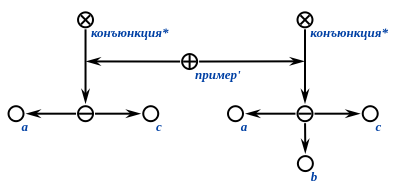
\includegraphics[scale=0.8]{author/part2/figures/logic/conjunction.png}
	\caption{Формализация примера конъюнкции}
	\label{fig:conjunction}
\end{figure}

%logically incorrect figure
%\begin{figure}[H]
%	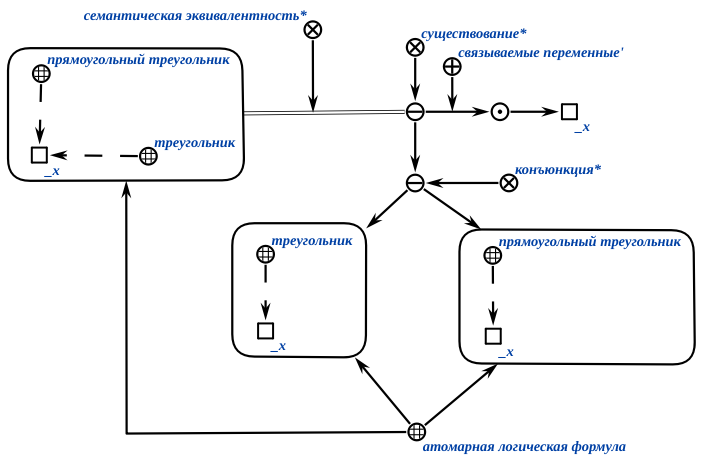
\includegraphics[scale=0.8]{author/part2/figures/logic/conjunction_triangles.png}
%	\caption{Формализация примера конъюнкции в геометрии}
%	\label{fig:conjunction_triangles}
%	\scnexplanation{Данные конструкции эквивалентны по принципу $\exists x T(x) \land \exists x PT(x) \ \Longrightarrow \ \exists x (T(x) \land PT(x))$}
%\end{figure}

\begin{SCn}
\scnheader{дизъюнкция*}
\scnidtf{логическое или*}
\scnidtf{логическое сложение*}
\scnidtf{включающее или*}
\scnsubset{логическая связка*}
\scniselement{неориентированное отношение}
\scniselement{класс связок разной мощности}
\scniselement{неунарное отношение}
\scnrelfrom{область определения}{логическая формула}
\end{SCn}

\textbf{\textit{дизъюнкция*}} --- это множество дизъюнктивных \textit{логических формул}, каждая из которых истинна (имеет истинные интерпретации) в рамках некоторой \textit{формальной теории} только в том случае, когда хотя бы один его компонент является истинным (имеет соответствующую истинную интерпретацию) в рамках этой же \textit{формальной теории}.

Следует отметить, что каждая конъюнктивная и дизъюнктивная формула представляют собой связку (множество) своих непосредственных подформул, причём эти множества могут быть равными, однако, такие множества будем полагать различными, так как одно множество будет представлять конъюнкцию, а другое -- дизъюнкцию. Наличие равных, но различных множеств не допускается в классической математике, которая основывается, в том числе, на абстракции обобщения (все равные множества (абстракции) -- тождественны). Однако, такие множества могут существовать в неклассических математических моделях. Таким образом, в рамках языка SC будем использовать неклассическую математическую модель для представления логических формул классической математической логики.

\begin{figure}[H]
	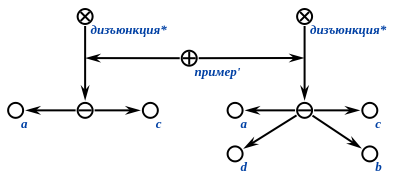
\includegraphics[scale=0.8]{author/part2/figures/logic/disjunction.png}
	\caption{Формализация примера дизъюнкции}
	\label{fig:disjunction}
\end{figure}

\begin{SCn}
\scnheader{отрицание*}
\scnsubset{логическая связка*}
\scnsubset{синглетон}
\scniselement{унарное отношение}
\scnrelfrom{область определения}{логическая формула}
\end{SCn}

\textbf{\textit{отрицание*}} --- это множество \textit{логических формул} об отрицании, каждое из которых истинно (имеет истинную интерпретацию) в рамках некоторой \textit{формальной теории} только в том случае, когда его единственный элемент является ложным (имеет ложную эту же интерпретацию) в рамках этой же \textit{формальной теории}.

\begin{figure}[H]
	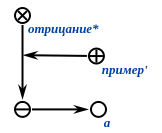
\includegraphics[scale=0.8]{author/part2/figures/logic/negation.png}
	\caption{Формализация примера отрицания}
	\label{fig:negation}
\end{figure}

\begin{SCn}
\scnheader{строгая дизъюнкция*}
%\scnidtf{сложение по модулю 2*}
\scnidtf{исключающее или*}
\scnidtf{альтернатива*}
\scnsubset{логическая связка*}
\scniselement{неориентированное отношение}
\scniselement{класс связок разной мощности}
\end{SCn}

\textbf{\textit{строгая дизъюнкция*}} --- это множество строго дизъюнктивных \textit{логических формул}, каждое из которых истинно в рамках некоторой \textit{формальной теории} только в том случае, когда ровно один его компонент является истинным (имеет соответствующую истинную интерпретацию) в рамках этой же \textit{формальной теории}.

\begin{figure}[H]
	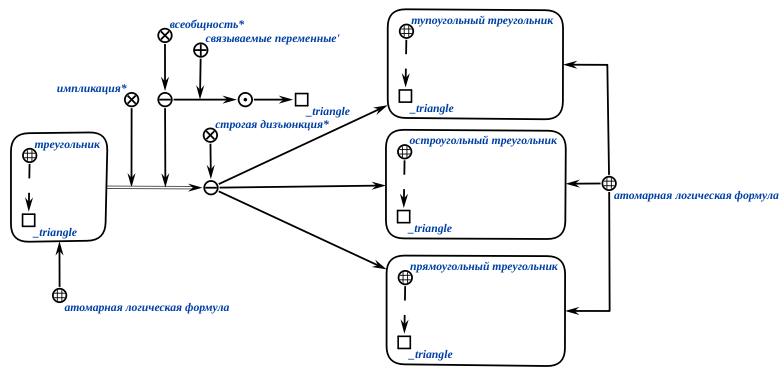
\includegraphics[scale=0.8]{author/part2/figures/logic/strict_disjunction_triangle.png}
	\caption{Формализация примера строгой дизъюнкции в геометрии}
	\label{fig:strict_disjunction_triangle}
\end{figure}
	\scnexplanation{Данная неатомарная логическая формула содержит следующую информацию: для любых переменных \_triangle если \_triangle является треугольником, то \_triangle является или тупоугольным треугольником, или остроугольным треугольником, или прямоугольным треугольником.}

\begin{figure}[H]
	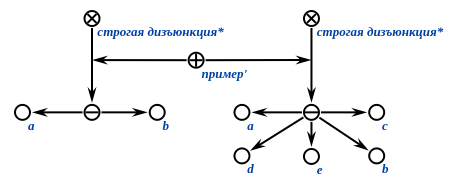
\includegraphics[scale=0.8]{author/part2/figures/logic/strictDisjunction.png}
	\caption{Формализация примера строгой дизъюнкции}
	\label{fig:strict_disjunction}
\end{figure}

\textbf{\textit{строгая дизъюнкция*}} может быть представлена как \textit{дизъюнкция} \textit{конъюнкции} \textit{отрицания} первой логической формулы и второй логической формулы и \textit{конъюнкции} первой логической формулы и \textit{отрицания} второй логической формулы. Также она может быть представлена и в виде \textit{конъюнкции} \textit{дизъюнкций} двух логических формул и их \textit{отрицаний}.

\begin{figure}[H]
	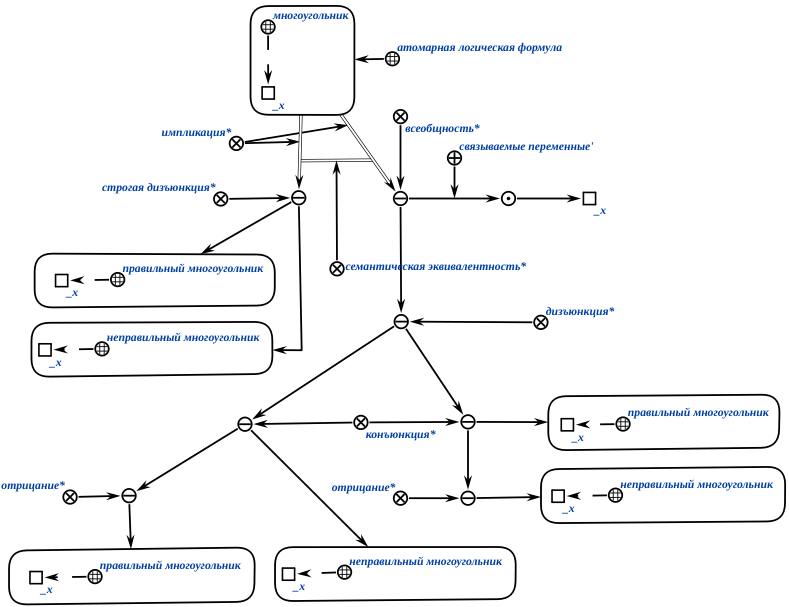
\includegraphics[scale=0.8]{author/part2/figures/logic/strict_disjunction_representation.png}
	\caption{Формализация примера строгой дизъюнкции}
	\label{fig:strict_disjunction_representation}
\end{figure}

\begin{SCn}
\scnheader{импликация*}
\scnidtf{логическое следование*}
\scnsubset{логическая связка*}
\scniselement{бинарное отношение}
\scniselement{ориентированное отношение}
\scnrelfrom{область определения}{логическая формула}
\end{SCn}

\textbf{\textit{импликация*}} --- это множество импликативных \textit{логических формул}, каждая из которых состоит из посылки (первый компонент \textit{высказывания}) и следствия (второй компонент \textit{высказывания}).

Каждое импликативное \textit{высказывание} ложно в рамках некоторой \textit{формальной теории} в том случае, когда его посылка истинна, а заключение ложно в рамках этой же \textit{формальной теории}. В других случаях такое \textit{высказывание} истинно.

По умолчанию на все переменные, входящие в обе части высказывания об \textbf{\textit{импликации*}} (или хотя бы одну из \textit{подформул*} каждой части) неявно накладывается квантор \textit{всеобщности*}, при условии, что эти переменные не связаны другим \textit{квантором}, указанным явно.

\begin{figure}[H]
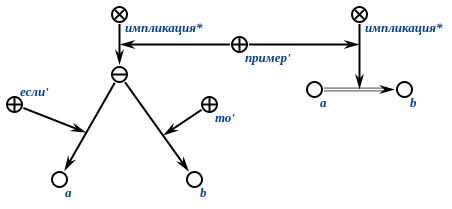
\includegraphics[scale=0.8]{author/part2/figures/logic/implication.png}
\caption{Формализация примера импликации}
\label{fig:implication}
\end{figure}

\textbf{\textit{импликация*}} может быть представлена как \textit{дизъюнкция} \textit{отрицания} первой логической формулы и второй логической формулы или же как \textit{отрицание} \textit{конъюнкции} первой логической формулы и \textit{отрицания} второй логической формулы.

\begin{figure}[H]
	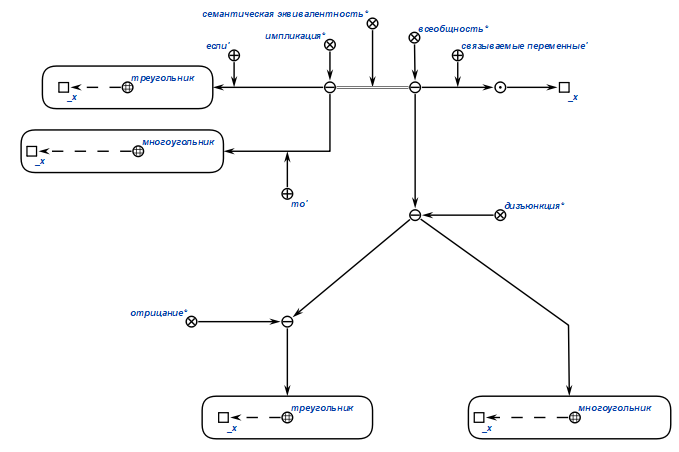
\includegraphics[scale=0.8]{author/part2/figures/logic/implication_representation.png}
	\caption{Формализация примера импликации}
	\label{fig:implication_representation}
\end{figure}

\begin{figure}[H]
	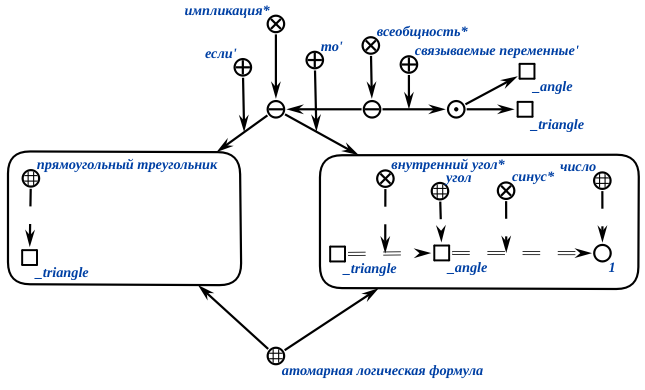
\includegraphics[scale=0.8]{author/part2/figures/logic/implication_triangle.png}
	\caption{Формализация примера импликации}
	\label{fig:implication_triangle}
\end{figure}
\vspace{-2\baselineskip}
\scnexplanation{Данная неатомарная логическая формула содержит следующую информацию: для любых переменных \_triangle и \_angle если \_triangle является прямоугольным треугольником, то синус его внутреннего угла \_angle равен единице.}

\begin{SCn}
\scnheader{если\scnrolesign}
\scnidtf{посылка\scnrolesign}
\scnsubset{1\scnrolesign}
\scniselement{ролевое отношение}
\end{SCn}

\textbf{\textit{если\scnrolesign}} --- это \textit{ролевое отношение}, используемое в связках \textit{импликации*} для указания посылки.

\begin{SCn}
\scnheader{то\scnrolesign}
\scnidtf{следствие\scnrolesign}
\scnsubset{2\scnrolesign}
\scniselement{ролевое отношение}
\end{SCn}

\textbf{\textit{то\scnrolesign}} --- это \textit{ролевое отношение}, используемое в связках \textit{импликации*} для указания следствия.

\begin{SCn}
\scnheader{эквиваленция*}
\scnidtf{эквивалентность*}
\scnsubset{логическая связка*}
\scniselement{бинарное отношение}
\scniselement{неориентированное отношение}
\scnrelfrom{область определения}{логическая формула}
\end{SCn}

\textbf{\textit{эквиваленция*}} --- это множество \textit{логических формул} об эквивалентности, каждое из которых истинно (имеет истинную интерпретацию) в рамках некоторой \textit{формальной теории} только в тех случаях, когда оба его компонента одновременно либо истинны (имеют соответствующие истинные интерпретации) в рамках этой же \textit{формальной теории}, либо ложны (имеют соответствующие ложные интерпретации).

По умолчанию на все переменные, входящие в обе части высказывания об \textbf{\textit{эквиваленции*}} (или хотя бы одну из \textit{подформул*} каждой части) неявно накладывается квантор \textit{всеобщности*}, при условии, что эти переменные не связаны другим \textit{квантором}, указанным явно.

\begin{figure}[H]
	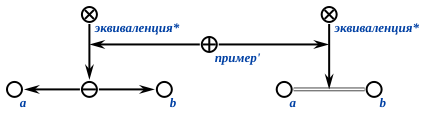
\includegraphics[scale=0.8]{author/part2/figures/logic/equivalent.png}
	\caption{Формализация примера эквиваленции}
	\label{fig:equivalent}
\end{figure}

\textbf{\textit{эквиваленция*}} двух логических формул может быть представлена как \textit{дизъюнкция} \textit{конъюнкции} этих двух логических формул и \textit{конъюнкции} \textit{отрицаний} этих двух логических формул.

\begin{figure}[H]
	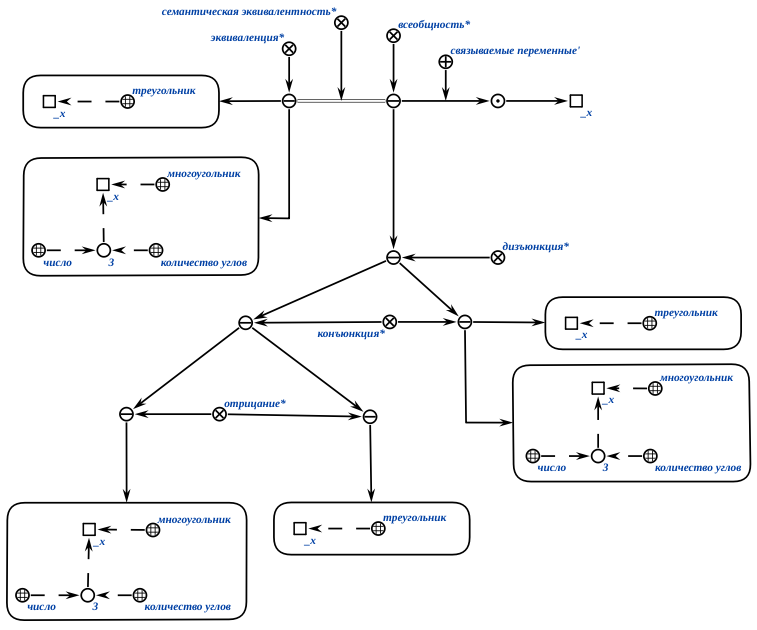
\includegraphics[scale=0.8]{author/part2/figures/logic/equivalence_representation.png}
	\caption{Формализация примера эквиваленции}
	\label{fig:equivalence_representation}
\end{figure}

\begin{SCn}
\scnheader{квантор}
\scnsubset{логическая связка*}
\end{SCn}

\textbf{\textit{квантор}} — это \textit{отношение}, каждая связка которого истинна (или имеет истинную интерпретацию) при выполнении дополнительных условий, связанных с некоторыми из переменных, входящих в состав \textit{логических формул}, входящих в ее состав.

Будем говорить, что переменные связаны \textbf{\textit{квантором}} или попадают под область действия данного \textbf{\textit{квантора}} (имея в виду конкретную связку конкретного \textbf{\textit{квантора}}).

В состав каждой связки каждого \textbf{\textit{квантора}} входит \textit{атомарная формула}, являющаяся \textit{тривиальной структурой}, в которой перечислены переменные, связанные данным \textbf{\textit{квантором}}.

\begin{SCn}
\scnheader{всеобщность*}
\scnidtf{квантор всеобщности*}
\scnidtf{квантор общности*}
\scniselement{квантор}
\scniselement{ориентированное отношение}
\scniselement{класс связок разной мощности}
\end{SCn}

\textbf{\textit{всеобщность*}} --- это \textit{квантор}, для каждой связки которого, истинной в рамках некоторой \textit{формальной теории} (или имеющей истинную интерпретацию), выполняется следующее утверждение: все формулы, входящие в состав этой связки имеют соответствующую истинную интерпретацию в рамках этой же \textit{формальной теории} при всех (любых) возможных значениях всех элементов множества \textit{связываемых переменных\scnrolesign} входящего в эту связку.

Каждая связка \textit{квантора} \textbf{\textit{всеобщность*}} может быть представлена как \textit{конъюнкция*} (потенциально бесконечная) исходных \textit{логических формул}, входящих в состав этой связки, в каждой из которых все \textit{связанные переменные\scnrolesign} заменены на их возможные значения.

Квантор \textbf{\textit{всеобщности*}} зачастую обозначается ``$\forall$'' и читается как ``для всех'', ``для каждого'', ``для любого'' или ``все'', ``каждый'', ``любой''.

\begin{figure}[H]
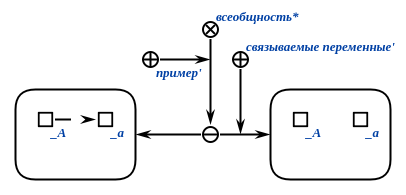
\includegraphics[scale=0.8]{author/part2/figures/logic/universality.png}
\caption{Формализация примера всеобщности}
\label{fig:universality}
\end{figure}

\begin{SCn}
\scnheader{формула существования}
\scnidtf{существование*}
\begin{scnrelfromset}{разбиение}
	\scnitem{атомарное существование}
	\scnitem{неатомарное существование*}
\end{scnrelfromset}

\scnheader{неатомарное существование*}
\scnidtf{квантор неатомарного существования*}
\scniselement{квантор}
\scniselement{ориентированное отношение}
\scniselement{класс связок разной мощности}
\end{SCn}

\textbf{\textit{неатомарное существование*}} --- это \textit{квантор}, для каждой связки которого, истинной в рамках некоторой \textit{формальной теории} (или имеющей истинную интерпретацию), выполняется следующее утверждение: существуют значения всех элементов множества \textit{связываемых переменных\scnrolesign} входящего в эту связку, такие, что все формулы, входящие в состав этой связки имеют соответствующую истинную интерпретацию в рамках этой же \textit{формальной теории}.

Каждая связка \textit{квантора} \textbf{\textit{неатомарное существование*}} может быть представлена как \textit{дизъюнкция*} (потенциально бесконечная) исходных \textit{логических формул}, входящих в состав этой связки, в каждой из которых все \textit{связанные переменные\scnrolesign} заменены на их возможные значения.

Квантор \textbf{\textit{существования*}} зачастую обозначается ``$\exists$'' и читается как ``существует'', ``для некоторого'', ``найдется''.

\begin{figure}[H]
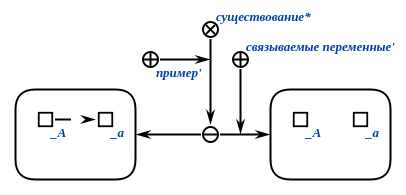
\includegraphics[scale=0.8]{author/part2/figures/logic/non_atomicExistence.png}
\caption{Формализация примера неатомарного существования}
\label{fig:non_atomic_existence}
\end{figure}

\begin{SCn}
\scnheader{число значений переменной}
\scniselement{параметр}
\end{SCn}

Каждый элемент \textit{параметра} \textbf{\textit{число значений переменной}} представляет собой класс ориентированных пар, первым компонентом которых является знак \textit{логической формулы}, вторым --- \textit{sc-переменная}, имеющая в рамках данной \textit{логической формулы} ограниченное известное число значений, при которых данная формула является истинной в рамках соответствующей \textit{формальной теории}.

Отметим, что в случае \textit{атомарной логической формулы} каждая такая связка связывает знак формулы и знак принадлежащей ей \textit{sc-переменной}, то есть является, по сути, частным случаем пары принадлежности. В случае \textit{неатомарной логической формулы} указанная \textit{sc-переменная} может принадлежать любой из \textit{подформул*} исходной формулы.

\textit{измерением*} значения параметра \textbf{\textit{число значений переменной}} является некоторое \textit{число}, задающее количество значений \textit{sc-переменных} в рамках \textit{логической формулы}.

\begin{SCn}
\scnheader{кратность существования}
\scniselement{параметр}
\scnrelfrom{область определения параметра}{формула существования}
\scnhaselement{единственное существование}
\end{SCn}

Каждый элемент \textit{параметра} \textbf{\textit{кратность существования}} представляет собой класс логических \textit{формул существования}, для которых  при интерпретации на соответствующей \textit{предметной области} существует ограниченное общее для всех таких формул число комбинаций значений переменных, при которых указанные формулы являются истинными в рамках соответствующей \textit{формальной теории}.
\textit{измерением*} каждого значения \textbf{\textit{кратности существования}} является некоторое \textit{число}, задающее количество таких комбинаций.

\begin{SCn}
\scnheader{единственное существование}
\scnidtf{однократное существование}
\scnidtf{формула существования и единственности}
\end{SCn}

Единственное существование зачастую обозначается ``$\exists!$'' и читается как ``существует и единственный''.

\begin{SCn}
\scnheader{логическая формула и единственность}
\scnsubset{логическая формула}
\scnsubset{единственное существование}
\end{SCn}

Каждый элемент множества \textbf{\textit{логическая формула и единственность}} представляет собой \textit{логическую формулу} (\textit{атомарную} или \textit{неатомарную}), для которой дополнительно уточняется, что при ее интерпретации на некоторой предметной области существует только один набор значений переменных, входящих в эту формулу (или ее \textit{подформулы*}), при котором указанная логическая формула истинна в рамках \textit{формальной теории}, в которую входит данная \textit{предметная область}.


%\scnfilescg{figures/sd_logical_formulas/unique_existance.png}
%Данная формула показывает, что в рамках формальной теории геометрии Евклида существует только один прямоугольный треугольник с некоторым периметром, являющийся равнобедренным.

\textbf{\textit{связываемые переменные\scnrolesign}} --- это \textit{ролевое отношение}, которое связывает связку конкретного \textit{квантора} с множеством переменных, которые связаны этим квантором.

\textbf{\textit{открытая логическая формула}} --- это \textit{логическая формула}, в рамках которой (и всех ее \textit{подформул*}) существует хотя бы одна переменная, не связанная никаким \textit{квантором}.

\textbf{\textit{замкнутая логическая формула}} --- это \textit{логическая формула}, в рамках которой (и всех ее \textit{подформул*}) не существует переменных, не связанных каким-либо \textit{квантором}.

%\scnheader{Примеры неатомарных логических формул}
%\scneqtoset{\scgfileitem{figures/sd_logical_formulas/example_line_segment_sum.png}\\
%\scnrelfrom{описание примера}{
%\scnfilescg{figures/sd_logical_formulas/example_line_segment_sum_note.png}}
%\scnexplanation{AB+BC=AC}
%;
%\scgfileitem{figures/sd_logical_formulas/example_line_segment_diff.png}\\
%\scnrelfrom{описание примера}{
%\scnfilescg{figures/sd_logical_formulas/example_line_segment_diff_note.png}}
%\scnexplanation{AB-AC=CB}

\section{Смысловое представление логических формул и высказываний в прикладных логиках}
\label{sec_applied_logic}
\begin{SCn}
	\begin{scnrelfromlist}{ключевое понятие}
		\scnitem{иррефлексивное слотовое бинарное отношение}
		\scnitem{иррефлексивное неслотовое бинарное отношение}
		\scnitem{рефлексивное слотовое бинарное отношение}
		\scnitem{рефлексивное неслотовое бинарное отношение}
		\scnitem{транзитивное слотовое бинарное отношение}
		\scnitem{транзитивное неслотовое бинарное отношение}
		\scnitem{симметричное слотовое бинарное отношение}
		\scnitem{симметричное неслотовое бинарное отношение}
		\scnitem{антисимметричное слотовое бинарное отношение}
		\scnitem{антисимметричное неслотовое бинарное отношение}
		\scnitem{монотонное бинарное отношение*}
		\scnitem{отношение порядка монотонного отношения\scnrolesign}
		\scnitem{монотонное бинарное отношение\scnrolesign}
		\scnitem{монотонное слотовое бинарное отношение*}
		\scnitem{монотонное неслотовое бинарное отношение*}
		\scnitem{слотовое бинарное отношение}
		\scnitem{неслотовое бинарное отношение}
		\scnitem{слотовое отношение эквивалентности}
		\scnitem{неслотовое отношение эквивалентности}
		\scnitem{слотовое отношение нестрогого порядка}
		\scnitem{неслотовое отношение нестрогого порядка}
		\scnitem{секвенция}
		\scnitem{метаструктура}
		\scnitem{модальный оператор}
		\scnitem{модальное правило вывода}
		\scnitem{отношение становления структур}
		\scnitem{последовательность мышления}
		\scnitem{последовательность рационального мышления}
		\scnitem{последовательность иррационального мышления}
		\scnitem{последовательность рационального мышления классической логики}
		\scnitem{последовательность рационального дедуктивного мышления классической логики}
		\scnitem{последовательность рационального дедуктивного мышления классической логики на конечных sc-множествах}
		\scnitem{последовательность классического рационального дедуктивного познания}
	\end{scnrelfromlist}
\end{SCn}
\begin{SCn}
	\begin{scnrelfromlist}{ключевой знак}
		\scnitem{Отношение выводимости}
		\scnitem{Отношение выводимости на конечных множествах}
		\scnitem{Отношение выводимости на конечных множествах полносвязно представленных множеств}
		\scnitem{Отношение выводимости на секвенциях}
	\end{scnrelfromlist}
\end{SCn}

Прикладные логики (см. \scncite{Klini1973}, \scncite{Gribomon1990}, \scncite{Dragalin}, \scncite{Vagin2008}, \scncite{Gribomon1998}, \scncite{Golenkov2001b}) рассматривают приложения классической логики к абстрактным и предметным областям, описывающим действительность: логические теории об отношениях равенства и порядка (см. \scncite{Klini1973}, \scncite{Gribomon1990}), логические теории арифметики (см. \scncite{Klini1973}), логические теории времени (см. \scncite{Gribomon1998}, \scncite{Vagin2008}), логические теории доказательств (см. \scncite{Dragalin}, \scncite{Klini1973}), теории графов и геометрические теории (см. \scncite{Golenkov2001b}), теории природных и социальных систем (см. \scncite{Gribomon1990}).

Классификация логических теорий соответствует классификации предметных областей.
Рассмотрим некоторые понятия и примеры, которые рассматриваются в рамках прикладных логик.

\begin{SCn}
	\scnheader{слотовое бинарное отношение}
	\scnnote{Слотовое бинарное отношение --- слотовое sc-отношение, являющееся множеством.}
\end{SCn}
\begin{SCn}
	\scnheader{неслотовое бинарное отношение}
	\scnnote{Неслотовое бинарное отношение --- бинарное sc-отношение, являющееся множеством, но не являющееся слотовым sc-отношением.}
\end{SCn}
\begin{SCn}
	\scnheader{иррефлексивное слотовое бинарное отношение}
	\scnsubset{иррефлексивное бинарное отношение}
	\scnnote{Иррефлексивное слотовое бинарное отношение --- слотовое (бинарное) отношение, любая связка которого не является связкой,обозначенной петлевой дугой (дугой с совпадающим началом и концом).}
\end{SCn}
\begin{SCn}
	\scnheader{иррефлексивное неслотовое бинарное отношение}
	\scnsubset{иррефлексивное бинарное отношение}
	\scnnote{Иррефлексивное неслотовое бинарное отношение --- неслотовое бинарное sc-отношение, для любой связки которого её различные принадлежности являются принадлежностями различных элементов.}
\end{SCn}
\begin{SCn}
	\scnheader{рефлексивное слотовое бинарное отношение}
	\scnsubset{рефлексивное бинарное отношение}
	\scnnote{Рефлексивное слотовое бинарное отношение --- слотовое бинарное sc-отношение, для любого элемента связки которого найдётся связка, обозначенная петлевой дугой (дугой с совпадающим началом и концом).}
\end{SCn}
\begin{SCn}
	\scnheader{рефлексивное неслотовое бинарное отношение}
	\scnsubset{рефлексивное бинарное отношение}
	\scnnote{Рефлексивное неслотовое бинарное отношение --- неслотовое бинарное sc-отношение, для любого элемента связки которого найдётся связка, имеющая две различные принадлежности этого элемента.}
\end{SCn}
\begin{SCn}
	\scnheader{транзитивное слотовое бинарное отношение}
	\scnsubset{транзитивное бинарное отношение}
	\scnnote{Транзитивное слотовое бинарное отношение --- слотовое бинарное отношение, для любых двух связок которого, конец одной из которых является началом второй, существует связка началом которой является начало первой связки, а концом является конец второй связки.}
\end{SCn}
\begin{SCn}
	\scnheader{транзитивное неслотовое бинарное отношение}
	\scnsubset{транзитивное бинарное отношение}
	\scnnote{Транзитивное неслотовое бинарное отношение --- неслотовое бинарное отношение, для которого существует ролевое отношение, первым доменом которого является это бинарное отношение такое, что для любых двух связок этого бинарного отношения, принадлежность элемента одной из которых не принадлежит этому ролевому отношению, а принадлежность этого же элемента второй связке принадлежит этому ролевому отношению, существует связка с принадлежностью элемента, принадлежащей ролевому отношению, принадлежность которого первой связке принадлежит ролевому отношению, и с принадлежностью элемента, не принадлежащей ролевому отношению, принадлежность которого второй связке не принадлежит этому ролевому отношению.}
\end{SCn}
\begin{SCn}
	\scnheader{симметричное слотовое бинарное отношение}
	\scnsubset{симметричное бинарное отношение}
	\scnnote{Симметричное слотовое бинарное отношение --- слотовое бинарное отношение, для любой связки которого существует связка, конец которой является началом первой связки, а начало --- её концом (т.е. эти связки обозначены встречными дугами).}
\end{SCn}
\begin{SCn}
	\scnheader{симметричное неслотовое бинарное отношение}
	\scnsubset{симметричное бинарное отношение}
	\scnnote{Симметричное неслотовое бинарное отношение --- неслотовое бинарное отношение, для которого существует ролевое отношение, первым доменом которого является это бинарное отношение, для любой связки которого существует связка с принадлежностью элемента первой связке, принадлежащая ролевому отношению, принадлежность которого второй связке не принадлежит этому ролевому отношению, и с принадлежностью элемента первой связке, не принадлежащая ролевому отношению, принадлежность которого второй связке принадлежит этому же ролевому отношению.}
\end{SCn}
\begin{SCn}
	\scnheader{антисимметричное слотовое бинарное отношение}
	\scnsubset{антисимметричное бинарное отношение}
	\scnnote{Антисимметричное слотовое бинарное отношение --- слотовое бинарное отношение, для любой связки которого у которой различным начало и конец не существует связки, конец которой является началом первой связки, а начало --- её концом (т.е. эти связки обозначены встречными дугами).}
\end{SCn}
\begin{SCn}
	\scnheader{антисимметричное неслотовое бинарное отношение}
	\scnsubset{антисимметричное бинарное отношение}
	\scnnote{Антисимметричное неслотовое бинарное отношение --- неслотовое бинарное отношение, для которого существует ролевое отношение, первым доменом которого является это бинарное отношение, для любой связки которого не существует связки с принадлежностью элемента первой связке, принадлежащая ролевому отношению, принадлежность которого второй связке не принадлежит этому ролевому отношению, и с принадлежностью другого элемента первой связке, не принадлежащая ролевому отношению, принадлежность которого второй связке принадлежит этому же ролевому отношению.}
\end{SCn}
\begin{SCn}
	\scnheader{монотонное слотовое бинарное отношение*}
	\scnsubset{монотонное бинарное отношение*}
	\scnnote{Монотонное слотовое бинарное отношение* --- слотовое бинарное отношение по отношению к отношению порядка, если есть связка этого бинарного отношения, то для любой его связки, начало которой связано связкой этого отношения порядка с началом первой, найдётся третья связка бинарного отношения, начало которой совпадает с началом втором связки, а конец совпадает с концом первой.}
\end{SCn}
\begin{SCn}
	\scnheader{отношение порядка монотонного отношения\scnrolesign}
	\scnrelfrom{первый домен}{монотонное бинарное отношение*}
	\scnrelfrom{второй домен}{отношение порядка}
\end{SCn}
\begin{SCn}
	\scnheader{монотонное бинарное отношение\scnrolesign}
	\scnrelfrom{первый домен}{монотонное бинарное отношение*}
	\scnrelfrom{второй домен}{монотонное бинарное отношение}
\end{SCn}
\begin{SCn}
	\scnheader{монотонное неслотовое бинарное отношение*}
	\scnsubset{монотонное бинарное отношение*}
	\scnnote{Монотонное неслотовое бинарное отношение* --- неслотовое бинарное отношение по отношению к отношению порядка, для которого существует ролевое отношение, первым доменом которого является это бинарное отношение, такое, что если есть связка этого бинарного отношения, то для любой его связки элемент принадлежащий ей под этим ролевым отношением в отличие от другого связан связкой этого отношения порядка с элементом принадлежащим первой связки под этим же ролевым отношением, в отличие от другого элемента первой связки, найдётся третья связка бинарного отношения такая, что элемент, принадлежащий ей под ролевым отношением, принадлежит под этим же ролевым отношением второй связке, а элемент, принадлежащий не под ролевым отношением третьей связке, принадлежит не под ролевым отношением первой связке.}
\end{SCn}
\begin{SCn}
	\scnheader{слотовое отношение эквивалентности}
	\scnsubset{sc-отношение эквивалентности}
	\scnnote{Слотовое отношение эквивалентности --- слотовое транзитивное бинарное отношение, которое является слотовым рефлексивным и симметричным отношением.}
\end{SCn}
\begin{SCn}
	\scnheader{неслотовое отношение эквивалентности}
	\scnsubset{sc-отношение эквивалентности}
	\scnnote{Неслотовое отношение эквивалентности --- неслотовое транзитивное бинарное отношение, которое является неслотовым рефлексивным и симметричным отношением (по соответствующим доменам).}
\end{SCn}
\begin{SCn}
	\scnheader{слотовое отношение нестрогого порядка}
	\scnsubset{sc-отношение нестрогого порядка}
	\scnnote{Слотовое отношение нестрогого порядка --- транзитивное бинарное отношение, которое является рефлексивным и антисимметричным.}
\end{SCn}
\begin{SCn}
	\scnheader{неслотовое отношение нестрогого порядка}
	\scnsubset{sc-отношение нестрогого порядка}
	\scnnote{Неслотовое отношение нестрогого порядка --- транзитивное бинарное отношение, которое является рефлексивным и антисимметричным (по соответствующим доменам).}
\end{SCn}

\begin{SCn}
	\scnheader{Отношение выводимости}
	\scnsuperset{Отношение выводимости на конечных множествах}
	\begin{scnindent}
		\scnsuperset{Отношение выводимости на конечных множествах полносвязно представленных множеств}
	\end{scnindent}
	\scniselement{рефлексивное бинарное отношение}
	\scniselement{транзитивное бинарное отношение}
	\scniselement{монотонное бинарное отношение}	
	\scnnote{Отношение выводимости --- рефлексивное, транзитивное, монотонное бинарное отношение на множествах посылок (высказываний, логических формул). Свойствами отношения выводимости являются правила вывода по Генцену.}
\end{SCn}

\begin{SCn}
	\scnheader{секвенция}
	\scnnote{секвенция --- связка (импликативного вида) между конъюнктивным множеством логических формул (конъюнкцией) и дизъюнктивным множеством логических формул (дизъюнкцией). Примером секвенции является выражение вида: $A_{1} \wedge A_{2} \wedge ... \wedge A_{n} \Rightarrow \ C_{1} \vee C_{2} \vee ... \vee C_{m}$.}
\end{SCn}

\begin{SCn}
	\scnheader{антецедент\scnrolesign}
	\scnrelfrom{первый домен}{секвенция}
	\scnrelfrom{второй домен}{конъюнкция}
\end{SCn}

\begin{SCn}
	\scnheader{консеквент\scnrolesign}
	\scnrelfrom{первый домен}{секвенция}
	\scnrelfrom{второй домен}{дизъюнкция}
\end{SCn}

\begin{SCn}
	\scnheader{Отношение выводимости на секвенциях}
	\scnnote{Отношение выводимости на секвенциях удовлетворяет правилам вывода исчисления секвенций.}
\end{SCn}

\begin{SCn}
	\scnheader{метаструктура}
	\scnnote{метаструктура --- структура, полносвязно представленным элементом которой является другая структура.}
\end{SCn}

\begin{SCn}
	\scnheader{модальный оператор}
	\scnnote{модальный оператор --- логическая связка, которая связывает логическую формулу со структурой (и иногда --- другими элементами) в метаструктуре. Примером модального оператора является оператор знания: $\mathrm{\Delta}$.}
\end{SCn}

\begin{SCn}
	\scnheader{модальное правило вывода}
	\scnnote{модальное правило вывода --- связка модального оператора формулы истинна (имеет истинную интерпретацию) в структуре, если и только если формула истинна (имеет истинную интерпретацию) в предшествующей ей структуре. Примером правила вывода является оператор знания: $\Gamma \cup \left\lbrace \alpha \right\rbrace \vdash \Gamma \cup \left\lbrace \mathrm{\Delta} \alpha \right\rbrace$.}
\end{SCn}

\begin{SCn}
	\scnheader{отношение становления структур}
	\scnnote{Отношение становления структур --- бинарное отношение на множестве структур, имеющих непустой общий носитель. Ролями в связке отношения становления являются ролевые отношения предшествующей структуры и последующей структуры.}
\end{SCn}

\begin{SCn}
	\scnheader{последовательность мышления}
	\scnidtf{судьба мышления}
	\scnidtf{мысль}	
	\scnnote{последовательность мышления --- последовательность sc-множеств высказываний (логических формул).}
	\begin{scnsubdividing}
		\scnitem{последовательность иррационального мышления}
		\scnitem{последовательность рационального мышления}
	\end{scnsubdividing}
\end{SCn}
\begin{SCn}
	\scnheader{последовательность рационального мышления классической логики}
	\scnidtf{судьба рационального мышления классической логики}
	\scnsubset{последовательность рационального мышления}
	\scnnote{последовательность рационального мышления --- последовательность (заданная отношением становления структур) (классически) непротиворечивых sc-множеств (sc-подмножеств или sc-надмножеств) высказываний.}
\end{SCn}
\begin{SCn}
	\scnheader{последовательность классического рационального дедуктивного мышления}
	\scnsubset{последовательность рационального мышления классической логики}
	\scnsuperset{последовательность рационального дедуктивного мышления классической логики на конечных sc-множествах}
	\scnnote{последовательность классического рационального дедуктивного мышления --- последовательность рационального мышления, последовательность (становления) непротиворечивых sc-множеств высказываний, дедуктивно логически следующих (по классическим правилам) друг за другом.}
\end{SCn}
\begin{SCn}
	\scnheader{последовательность классического рационального дедуктивного познания}
	\scnidtf{воля}
	\scnnote{последовательность классического рационального дедуктивного познания --- последовательность (заданная отношением становления структур) непротиворечивых sc-надмножеств высказываний, логически следующих друг за другом.}
\end{SCn}

\section{Смысловое представление логических формул и высказываний в неклассических логиках}
\label{sec_nonclass_logic}

\begin{SCn}
	\begin{scnrelfromlist}{ключевое понятие}
		\scnitem{немонотонный вывод на конечном sc-множестве посылок}
		\scnitem{выводимое множество}
		\scnitem{нечёткая истинность*}
		\scnitem{конструктивно истинное высказывание*}
		\scnitem{верное высказывание*}
		\scnitem{неискажённое высказывание*}
	\end{scnrelfromlist}
\end{SCn}

\textbf{\textit{неклассические логики}} (см. \scncite{Gribomon1990}, \scncite{Gribomon1998}, \scncite{Dragalin}, \scncite{Tarasov2007}, \scncite{Cintula2011}, \scncite{Vagin2008}) рассматривают (1) неклассический вывод, в котором отношение выводимости обладает иными свойствами (см. \scncite{Gribomon1990}, \scncite{Gribomon1998}, \scncite{Vagin2008}, \scncite{Dragalin}) и при котором можно или нельзя вывести то, что выводимо в классической логике, а также (2) --- другие шкалы признаков логических формул, их интерпретаций и значений (см. \scncite{Tarasov2007}, \scncite{Cintula2011}), отличных от ложных и (достоверно) истинных.

\begin{SCn}
	\scnheader{немонотонный вывод на конечном sc-множестве посылок*}
	\scnnote{\textit{немонотонный вывод на конечном sc-множестве посылок*} --- \textit{отношение} между (конечными) \textit{sc-множествами} истинных \textit{логических высказываний} (посылок). Если не существует вложения структуры \textit{атомарной логической формулы} в реляционную структуру (sc-подмножество предметной области) \textit{sc-множества} истинных (непротиворечивых) посылок и относительно них истинно отрицание этой \textit{атомарной формулы}, то существует \textit{sc-множество}, с принадлежащей ему реляционной структурой, включающей все элементы ранее упомянутой реляционной структуры и константы этой \textit{атомарной формулы}, которому принадлежат все посылки ранее упомянутого sc-множества истинных (непротиворечивых) посылок и упомянутая атомарная логическая формула.}
\end{SCn}

\begin{SCn}
	\scnheader{выводимое множество}
	\scnnote{\textit{выводимое множество} --- \textit{ситуативное sc-множество} (см. \scncite{Ivashenko2014diss}, \scncite{Ivashenko2017}), (временная) принадлежность \textit{логических формул} которому устанавливается в порядке становления процесса вывода этих \textit{логических формул}.}
\end{SCn}

\begin{SCn}
	\scnheader{нечёткая истинность*}
	\scnnote{\textit{нечёткая истинность*} связывает конечное sc-множество с временными принадлежностями на конечном множестве конечных явлений принадлежности с высказыванием. На явлениях принадлежности задано конечное sc-подмножество sc-отношения становления (непосредственно прежде, непосредственно после), которое задаёт структуру соответствующих sc-подмножеств. Эта структура является ориентированным деревом. \textit{нечёткая истинность*} --- \textit{бинарное отношение} между (нечёткой) принадлежностью связки  \textit{высказывания} \textit{формальной теории} и конечного sc-множества и действительным числом от 0.0 до 1.0. Нечёткая истинность отрицания высказывания равна разности 1.0 и нечёткой истинности высказывания, принадлежащего отрицанию. \textit{нечёткая истинность*} \textit{конъюнкции*} высказываний не превышает минимума нечёткой истинности элементов этой конъюнкции и не ниже (граничного или драстического) произведения \textit{нечёткой истинности*} этих же элементов конъюнкции. 
	\textit{нечёткая истинность*} \textit{дизъюнкции*} не превышает (граничной или драстической) суммы \textit{нечёткой истинности*} элементов этой конъюнкции и не ниже максимума нечёткой истинности этих же элементов конъюнкции.
	\textit{нечёткая истинность*} \textit{атомарных высказываний} равна среднему арифметическому изоморфного вложения структуры \textit{высказывания} в каждое из sc-подмножеств конечного sc-множества, которые входят в структуру заданную sc-отношением становления.}
\end{SCn}

\begin{SCn}
	\scnheader{конструктивно истинное высказывание*}
	\scnnote{\textbf{\textit{конструктивно истинное высказывание*}} --- подмножество \textit{истинного высказывания*}. 
	Истинные \textit{атомарные логические формулы} или их истинные интерпретации --- конструктивно истинные, если и только если они имеют изоморфное вложение в предметную область, где все элементы вложения полносвязно представлены. 
	\textit{конъюнкция*} \textit{конструктивно истинных логических формул} (или имеющих соответствующие конструктивно истинные интерпретации) конструктивно истинна (или имеет конструктивно истинную соответствующую интерпретацию).
	\textit{дизъюнкция*} хотя бы одной \textit{конструктивно истинной логической формулы} (или имеющей соответствующую полную конструктивно истинную интерпретацию) конструктивно истинна (или имеет конструктивно истинную соответствующую интерпретацию).
	\textit{отрицание*} \textit{ложной логической формулы} (или имеющей ложную соответствующую интерпретацию) конструктивно истинное (или имеет конструктивно истинную интерпретацию).
	Если все \textit{логические формулы} в \textit{дизъюнкции*} ложны (имеют соответствующие ложные интерпретации), то и дизъюнкция ложна (имеет соответствующую ложную интерпретацию).
	\textit{отрицание*} \textit{ложной логической формулы} (или имеющей ложную соответствующую интерпретацию) конструктивно истинное (или имеет конструктивно истинную интерпретацию).
	\textit{импликация*} с ложной посылкой (или имеющей соответствующую ложную интерпретацию) конструктивна истинна (или имеет конструктивно истинную интерпретацию).
	\textit{импликация*} с конструктивно истинным следствием (или имеющим соответствующую конструктивно истинную интерпретацию) конструктивна истинна (или имеет конструктивно истинную интерпретацию).
	\textit{конструктивно истинная импликация*} (или имеющая конструктивно истинную интерпретацию) с конструктивно истинной посылкой (или имеющей соответствующую конструктивно истинную интерпретацию) имеет конструктивно истинное следствие (или имеющее соответствующую конструктивно истинную интерпретацию).
	\textit{конструктивно истинная импликация*} (или имеющая конструктивно истинную интерпретацию) с ложным следствием (или имеющим соответствующую ложную интерпретацию) имеет ложную посылку (или имеющую соответствующую ложную интерпретацию).
	Существование значений переменных для \textit{логической формулы} конструктивно истинно (или имеет соответствующую конструктивную истинную интерпретацию), если всеобщность значений переменных для этой \textit{логической формулы} конструктивно истинна (или имеет соответствующую конструктивную истинную интерпретацию).
	Если \textit{логическая формула} имеет только конструктивно истинные соответствующие интерпретации, то всеобщность значений переменной для этой \textit{логической формулы} конструктивно истинна (или имеет соответствующую конструктивно истинную интерпретацию).
}
\end{SCn}

\begin{SCn}
	\scnheader{верное высказывание*}
	\scnnote{\textit{верное высказывание*} --- \textit{высказывание}, которое является истинным или неискажённым.}	
\end{SCn}

\begin{SCn}
	\scnheader{неискажённое высказывание*}
	\scnnote{\textit{неискажёное высказывание*} --- \textit{высказывание}, верность или неверность которого не приводит к противоречию.}	
\end{SCn}

%%%%%%%%%%%%%%%%%%%%%%%%% referenc.tex %%%%%%%%%%%%%%%%%%%%%%%%%%%%%%
% sample references
% %
% Use this file as a template for your own input.
%
%%%%%%%%%%%%%%%%%%%%%%%% Springer-Verlag %%%%%%%%%%%%%%%%%%%%%%%%%%
%
% BibTeX users please use
% \bibliographystyle{}
% \bibliography{}
%
\biblstarthook{In view of the parallel print and (chapter-wise) online publication of your book at \url{www.springerlink.com} it has been decided that -- as a genreral rule --  references should be sorted chapter-wise and placed at the end of the individual chapters. However, upon agreement with your contact at Springer you may list your references in a single seperate chapter at the end of your book. Deactivate the class option \texttt{sectrefs} and the \texttt{thebibliography} environment will be put out as a chapter of its own.\\\indent
References may be \textit{cited} in the text either by number (preferred) or by author/year.\footnote{Make sure that all references from the list are cited in the text. Those not cited should be moved to a separate \textit{Further Reading} section or chapter.} If the citatiion in the text is numbered, the reference list should be arranged in ascending order. If the citation in the text is author/year, the reference list should be \textit{sorted} alphabetically and if there are several works by the same author, the following order should be used:
\begin{enumerate}
\item all works by the author alone, ordered chronologically by year of publication
\item all works by the author with a coauthor, ordered alphabetically by coauthor
\item all works by the author with several coauthors, ordered chronologically by year of publication.
\end{enumerate}
The \textit{styling} of references\footnote{Always use the standard abbreviation of a journal's name according to the ISSN \textit{List of Title Word Abbreviations}, see \url{http://www.issn.org/en/node/344}} depends on the subject of your book:
\begin{itemize}
\item The \textit{two} recommended styles for references in books on \textit{mathematical, physical, statistical and computer sciences} are depicted in ~\cite{science-contrib, science-online, science-mono, science-journal, science-DOI} and ~\cite{phys-online, phys-mono, phys-journal, phys-DOI, phys-contrib}.
\item Examples of the most commonly used reference style in books on \textit{Psychology, Social Sciences} are~\cite{psysoc-mono, psysoc-online,psysoc-journal, psysoc-contrib, psysoc-DOI}.
\item Examples for references in books on \textit{Humanities, Linguistics, Philosophy} are~\cite{humlinphil-journal, humlinphil-contrib, humlinphil-mono, humlinphil-online, humlinphil-DOI}.
\item Examples of the basic Springer style used in publications on a wide range of subjects such as \textit{Computer Science, Economics, Engineering, Geosciences, Life Sciences, Medicine, Biomedicine} are ~\cite{basic-contrib, basic-online, basic-journal, basic-DOI, basic-mono}. 
\end{itemize}
}

\begin{thebibliography}{99.}%
% and use \bibitem to create references.
%
% Use the following syntax and markup for your references if 
% the subject of your book is from the field 
% "Mathematics, Physics, Statistics, Computer Science"
%
% Contribution 
\bibitem{science-contrib} Broy, M.: Software engineering --- from auxiliary to key technologies. In: Broy, M., Dener, E. (eds.) Software Pioneers, pp. 10-13. Springer, Heidelberg (2002)
%
% Online Document
\bibitem{science-online} Dod, J.: Effective substances. In: The Dictionary of Substances and Their Effects. Royal Society of Chemistry (1999) Available via DIALOG. \\
\url{http://www.rsc.org/dose/title of subordinate document. Cited 15 Jan 1999}
%
% Monograph
\bibitem{science-mono} Geddes, K.O., Czapor, S.R., Labahn, G.: Algorithms for Computer Algebra. Kluwer, Boston (1992) 
%
% Journal article
\bibitem{science-journal} Hamburger, C.: Quasimonotonicity, regularity and duality for nonlinear systems of partial differential equations. Ann. Mat. Pura. Appl. \textbf{169}, 321--354 (1995)
%
% Journal article by DOI
\bibitem{science-DOI} Slifka, M.K., Whitton, J.L.: Clinical implications of dysregulated cytokine production. J. Mol. Med. (2000) doi: 10.1007/s001090000086 
%
\bigskip

% Use the following (APS) syntax and markup for your references if 
% the subject of your book is from the field 
% "Mathematics, Physics, Statistics, Computer Science"
%
% Online Document
\bibitem{phys-online} J. Dod, in \textit{The Dictionary of Substances and Their Effects}, Royal Society of Chemistry. (Available via DIALOG, 1999), 
\url{http://www.rsc.org/dose/title of subordinate document. Cited 15 Jan 1999}
%
% Monograph
\bibitem{phys-mono} H. Ibach, H. L\"uth, \textit{Solid-State Physics}, 2nd edn. (Springer, New York, 1996), pp. 45-56 
%
% Journal article
\bibitem{phys-journal} S. Preuss, A. Demchuk Jr., M. Stuke, Appl. Phys. A \textbf{61}
%
% Journal article by DOI
\bibitem{phys-DOI} M.K. Slifka, J.L. Whitton, J. Mol. Med., doi: 10.1007/s001090000086
%
% Contribution 
\bibitem{phys-contrib} S.E. Smith, in \textit{Neuromuscular Junction}, ed. by E. Zaimis. Handbook of Experimental Pharmacology, vol 42 (Springer, Heidelberg, 1976), p. 593
%
\bigskip
%
% Use the following syntax and markup for your references if 
% the subject of your book is from the field 
% "Psychology, Social Sciences"
%
%
% Monograph
\bibitem{psysoc-mono} Calfee, R.~C., \& Valencia, R.~R. (1991). \textit{APA guide to preparing manuscripts for journal publication.} Washington, DC: American Psychological Association.
%
% Online Document
\bibitem{psysoc-online} Dod, J. (1999). Effective substances. In: The dictionary of substances and their effects. Royal Society of Chemistry. Available via DIALOG. \\
\url{http://www.rsc.org/dose/Effective substances.} Cited 15 Jan 1999.
%
% Journal article
\bibitem{psysoc-journal} Harris, M., Karper, E., Stacks, G., Hoffman, D., DeNiro, R., Cruz, P., et al. (2001). Writing labs and the Hollywood connection. \textit{J Film} Writing, 44(3), 213--245.
%
% Contribution 
\bibitem{psysoc-contrib} O'Neil, J.~M., \& Egan, J. (1992). Men's and women's gender role journeys: Metaphor for healing, transition, and transformation. In B.~R. Wainrig (Ed.), \textit{Gender issues across the life cycle} (pp. 107--123). New York: Springer.
%
% Journal article by DOI
\bibitem{psysoc-DOI}Kreger, M., Brindis, C.D., Manuel, D.M., Sassoubre, L. (2007). Lessons learned in systems change initiatives: benchmarks and indicators. \textit{American Journal of Community Psychology}, doi: 10.1007/s10464-007-9108-14.
%
%
% Use the following syntax and markup for your references if 
% the subject of your book is from the field 
% "Humanities, Linguistics, Philosophy"
%
\bigskip
%
% Journal article
\bibitem{humlinphil-journal} Alber John, Daniel C. O'Connell, and Sabine Kowal. 2002. Personal perspective in TV interviews. \textit{Pragmatics} 12:257--271
%
% Contribution 
\bibitem{humlinphil-contrib} Cameron, Deborah. 1997. Theoretical debates in feminist linguistics: Questions of sex and gender. In \textit{Gender and discourse}, ed. Ruth Wodak, 99--119. London: Sage Publications.
%
% Monograph
\bibitem{humlinphil-mono} Cameron, Deborah. 1985. \textit{Feminism and linguistic theory.} New York: St. Martin's Press.
%
% Online Document
\bibitem{humlinphil-online} Dod, Jake. 1999. Effective substances. In: The dictionary of substances and their effects. Royal Society of Chemistry. Available via DIALOG. \\
http://www.rsc.org/dose/title of subordinate document. Cited 15 Jan 1999
%
% Journal article by DOI
\bibitem{humlinphil-DOI} Suleiman, Camelia, Daniel C. O'Connell, and Sabine Kowal. 2002. `If you and I, if we, in this later day, lose that sacred fire...': Perspective in political interviews. \textit{Journal of Psycholinguistic Research}. doi: 10.1023/A:1015592129296.
%
%
%
\bigskip
%
%
% Use the following syntax and markup for your references if 
% the subject of your book is from the field 
% "Computer Science, Economics, Engineering, Geosciences, Life Sciences"
%
%
% Contribution 
\bibitem{basic-contrib} Brown B, Aaron M (2001) The politics of nature. In: Smith J (ed) The rise of modern genomics, 3rd edn. Wiley, New York 
%
% Online Document
\bibitem{basic-online} Dod J (1999) Effective Substances. In: The dictionary of substances and their effects. Royal Society of Chemistry. Available via DIALOG. \\
\url{http://www.rsc.org/dose/title of subordinate document. Cited 15 Jan 1999}
%
% Journal article by DOI
\bibitem{basic-DOI} Slifka MK, Whitton JL (2000) Clinical implications of dysregulated cytokine production. J Mol Med, doi: 10.1007/s001090000086
%
% Journal article
\bibitem{basic-journal} Smith J, Jones M Jr, Houghton L et al (1999) Future of health insurance. N Engl J Med 965:325--329
%
% Monograph
\bibitem{basic-mono} South J, Blass B (2001) The future of modern genomics. Blackwell, London 
%
\end{thebibliography}
